\begin{ex}%Cau12D%[2D4H2-6]
Một ô tô đang dừng và bắt đầu chuyển động theo một đường thẳng với gia tốc $a\left(t\right)= 6-2t$ (m/s$^2$), trong đó $t$ là khoảng thời gian tính bằng giây kể từ lúc ô tô bắt đầu chuyển động. Hỏi quảng đường ô tô đi được từ lúc bắt đầu chuyển động đến khi vận tốc của ô tô đạt giá trị lớn nhất là bao nhiêu mét?
\choice
	{\True $18$ m}
	{$36$ m}
	{$22{,}5$ m}
	{$6{,}75$ m}
	\loigiai{
	$a\left(t\right) = 6-2t$ (m/s$^2$) $\Rightarrow v\left(t\right) = \displaystyle\int \left(6-2t\right) \mathrm{\,d}t = 6t - t^2+C$.\\
	Xe dừng và bắt đầu chuyển động nên khi $t=0$ thì $v=0 \Rightarrow C=0 \Rightarrow v\left(t\right) = 6t-t^2$.\\
	$v\left(t\right) = 6t-t^2$ là hàm số bậc $2$ nên đạt giá trị lớn nhất khi $t=-\dfrac{b}{2a}=3$ (s).\\
	Quãng đường xe đi trong $3$ giây đầu là: $S= \displaystyle\int\limits_0^3 \left(6t-t^2\right) \mathrm{\,d}t = 18$ (m).
	}
\end{ex}

\begin{ex}%Cau13D%[2D4V2-6]
Một chất điểm $A$ xuất phát từ $O$, chuyển động thẳng với vận tốc biến thiên theo thời gian bởi quy luật $v \left(t\right) = \dfrac{1}{180}t^2 + \dfrac{11}{18}t$ (m/s), trong đó $t$ (giây) là khoảng thời gian tính từ lúc $A$ bắt đầu chuyển động. Từ trạng thái nghỉ, một chất điểm $B$ cũng xuất phát từ $O$, chuyển động thẳng cùng hướng với $A$ nhưng chậm hơn $5$ giây so với $A$ và có gia tốc bằng $a$ (m/s$^2$) ($a$ là hằng số). Sau khi $B$ xuất phát được $10$ giây thì đuổi kịp $A$. Vận tốc của $B$ tại thời điểm đuổi kịp $A$ bằng
\choice
	{\True $15$ (m/s)}
	{$10$ (m/s)}
	{$7$ (m/s)}
	{$22$(m/s)}
	\loigiai{
	Thời gian tính từ khi $A$ xuất phát đến khi bị $B$ đuổi kịp là $15$ giây, suy ra quãng đường đi được tới lúc đó là:
	$$\displaystyle\int\limits_0^{15} v\left(t\right) \mathrm{\,d}t = \displaystyle\int\limits_0^{15} \left(\dfrac{1}{180}t^2 + \dfrac{11}{18}t \right) \mathrm{\,d}t= \left(\dfrac{1}{540}t^3 + \dfrac{11}{36}t^2 \right)\Big|_0^{15} = 75 \left(\text{m}\right).$$
Vận tốc của chất điểm $B$ là $y\left(t\right) = \displaystyle\int a \mathrm{\,d}t = a \cdot t+C$ ( $C$ là hằng số); do $B$ xuất phát từ trạng thái nghỉ nên có $y\left(0\right)=0 \Leftrightarrow C=0$.\\
Quãng đường của $B$ từ khi xuất phát đến khi đuổi kịp $A$ là
$$\displaystyle\int\limits_0^{10} y\left(t\right) \mathrm{\,d}t = 75 \Leftrightarrow \displaystyle\int\limits_0^{10} a \cdot t \mathrm{\,d}t =75 \Leftrightarrow \dfrac{a \cdot t^2}{2}\Big|_0^{10} = 75 \Leftrightarrow 50a=75 \Leftrightarrow a = \dfrac{3}{2}.$$
Vậy có $y\left(t\right) = \dfrac{3t}{2}$; suy ra vận tốc của $B$ tại thời điểm đuổi kịp $A$ bằng $y\left(10\right) = 15$ (m/s).
	}
\end{ex}

\begin{ex}%Cau14D%[2D4V2-6]
Một vật chuyển động trong $3$ giờ với vận tốc $v$ (km/h) phụ thuộc thời gian $t$ (h) có đồ thị là một phần của đường parabol có đỉnh $I\left(2;9\right)$ và trục đối xứng song song với trục tung như hình bên. Tính quãng đường $s$ mà vật di chuyển được trong $3$ giờ đó.
\begin{center}
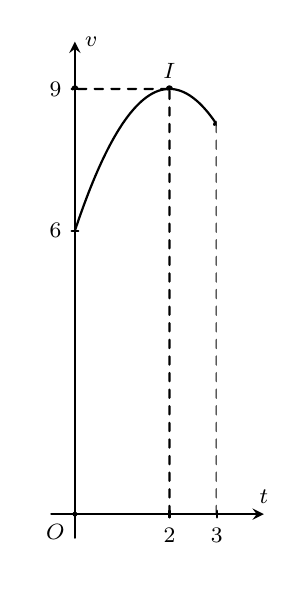
\begin{tikzpicture}[>=stealth, font=\footnotesize, line join=round, line cap=round, thick, smooth, samples=250, scale=0.6]
% Vẽ 2 trục, điền các số lên trục
 \draw[->] (-0.5,0)--(0,0) node[below left]{$O$}--(4,0) node[above]{$t$};
\foreach \x in {2,3}
\draw[shift={(\x,0)},color=black] (0pt,2pt)--(0pt,-2pt) 
node[below] { $\x$};
\draw[->,color=black] (0,-0.5)--(0,10) node[right]{$v$};
\foreach \y in {6,9}
\draw[shift={(0,\y)},color=black] (2pt,0pt) -- (-2pt,0pt) 
node[left] {$\y$};
\clip(-1,-1) rectangle (3,10); %vùng đồ thị
%\draw[gray!50,thin,opacity=.5] (-1,-1) grid (4,10); %ô vuông
%Vẽ đồ thị
\draw[smooth,samples=100,domain=0:10] 
plot(\x,{(-0.75)*(\x)^2+3*(\x)+6});
\draw[dashed] (3,0)--(3,8.25) circle(1.5pt);  \draw[dashed] (2,0)--(2,9) circle(1.5pt) node[above]{$I$}--(0,9) circle(1.5pt);
% Vẽ thêm mấy cái râu ria

%Vẽ dấu chấm tròn 
\fill (0cm,0cm) circle (1.5pt); 
\end{tikzpicture}
\end{center}
\choice
	{$s = 25{,}25$ (km)}
	{$s = 24{,}25$ (km)}
	{\True $s = 24{,}75$ (km)}
	{$s = 26{,}75$ (km)}
	\loigiai{Gọi $v \left(t\right) = at^2 +bt +c$.\\
	Đồ thị $v\left(t\right)$ là một phần parabol có đỉnh $I\left(2;9\right)$ và đi qua điểm $A\left(0;6\right)$ nên\\
	$\heva{&\dfrac{-b}{2a} = 2\\&a \cdot 2^2 +b\cdot 2 +c=9\\&a \cdot 0^2 + b \cdot 0+c =6} \Rightarrow \heva{&a = -\dfrac{3}{4}\\&b=3\\&c=6}$. Tìm được $v\left(t\right) = -\dfrac{3}{4}t^2 + 3t +6$.\\
	Vậy $S = \displaystyle\int\limits_0^{3} \left(-\dfrac{3}{4} t^2 + 3t +6 \right) \mathrm{\,d}t = 24{,}75$ (km).
	}
\end{ex}

\begin{ex}%Cau15D%[2D4H2-6]
Một vật chuyển động trong $3$ giờ với vận tốc $v$ (km/h) phụ thuộc vào thời gian $t$ (h) có đồ thị vận tốc như hình bên. Trong thời gian $1$ giờ kể từ khi bắt đầu chuyển động, đồ thị đó là một phần của đường parabol có đỉnh $I\left(2;9\right)$ và trục đối xứng song song với trục tung, khoảng thời gian còn lại đồ thị là một đoạn thẳng song song với trục hoành. Tính quãng đường $s$ mà vật chuyển động được trong $3$ giờ đó (kết quả làm tròn đến hàng phần trăm).
\begin{center}
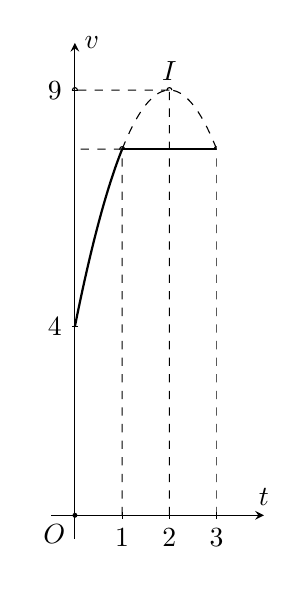
\begin{tikzpicture}[>=stealth,scale=0.6]
% Vẽ 2 trục, điền các số lên trục
 \draw[->] (-0.5,0)--(0,0) node[below left]{$O$}--(4,0) node[above]{$t$}; %định dạng trục Ox
\foreach \x in {1,2,3}
\draw[shift={(\x,0)},color=black] (0pt,2pt)--(0pt,-2pt) 
node[below] { $\x$};
\draw[->,color=black] (0,-0.5)--(0,10) node[right]{$v$};  %định dạng trục Oy
\foreach \y in {4,9}
\draw[shift={(0,\y)},color=black] (2pt,0pt) -- (-2pt,0pt) 
node[left] {$\y$};
\clip(-1,-1) rectangle (3,10); %vùng đồ thị
%\draw[gray!50,thin,opacity=.5] (-1,-1) grid (4,10); %ô vuông
%Vẽ đồ thị
\draw[smooth,samples=100,domain=0:1,font=\footnotesize, line join=round, line cap=round, thick] 
plot(\x,{(-5/4)*(\x)^2+5*(\x)+4});
\draw[smooth,samples=100,domain=1:3,dashed] 
plot(\x,{(-5/4)*(\x)^2+5*(\x)+4});
\draw[smooth,samples=100,domain=1:3,font=\footnotesize, line join=round, line cap=round, thick] 
plot(\x,{31/4});
% Vẽ thêm mấy cái râu ria
\draw[dashed] (3,0)--(3,31/4) circle(1.5pt);  \draw[dashed] (2,0)--(2,9) circle(1.5pt) node[above]{$I$}--(0,9) circle(1.5pt); \draw[dashed] (1,0)--(1,31/4) circle(1.5pt) --(0,31/4);
%Vẽ dấu chấm tròn 
\fill (0cm,0cm) circle (1.5pt); 
\end{tikzpicture}
\end{center}
\choice
	{\True $s = 21{,}58$ (km)}
	{$s = 23{,}25$ (km)}
	{$s = 13{,}83$ (km)}
	{$s = 15{,}50$ (km)}
	\loigiai{Gọi phương trình parabol $v = at^2+bt+c$ ta có hệ như sau
		$$\heva{&c=4\\&4a+2b+c=9\\&-\dfrac{b}{2a}=2} \Leftrightarrow \heva{&b=5\\&c=4\\&a=-\dfrac{5}{4}.}$$
	Với $t=1$ ta có $v = \dfrac{31}{4}$.
	Vậy quãng đường vật chuyển động được là
	$$s = \displaystyle\int\limits_0^1 \left(-\dfrac{5}{4}t^2 + 5t +4 \right) \mathrm{\,d}t + \displaystyle\int\limits_1^3 \dfrac{31}{4} \mathrm{\,d}t = \dfrac{259}{12} \approx 21{,}58.$$
	}
\end{ex}

\begin{ex} %Cau16D %[2D4H2-6]
Một người chạy trong $2$ giờ, vận tốc $v$ (km/h) phụ thuộc vào thời gian $t$ (h) có đồ thị là $1$ phần của đường Parabol với đỉnh $I\left(1;5\right)$ và trục đối xứng song song với trục tung $Ov$ như hình vẽ. Tính quảng đường $S$ người đó chạy được trong $1$ giờ $30$ phút kể từ lúc bắt đầu chạy (kết quả làm tròn đến $2$ chữ số thập phân).
\begin{center}
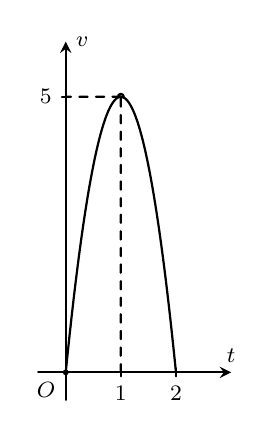
\begin{tikzpicture}[>=stealth, font=\footnotesize, line join=round, line cap=round, thick, smooth, samples=250, scale=0.7]
% Vẽ 2 trục, điền các số lên trục
 \draw[->] (-0.5,0)--(0,0) node[below left]{$O$}--(3,0) node[above]{$t$}; %định dạng trục Ox
\foreach \x in {2,1}
\draw[shift={(\x,0)},color=black] (0pt,2pt)--(0pt,-2pt) 
node[below] { $\x$};
\draw[->,color=black] (0,-0.5)--(0,6) node[right]{$v$};  %định dạng trục Oy
\foreach \y in {5}
\draw[shift={(0,\y)},color=black] (2pt,0pt) -- (-2pt,0pt) 
node[left] {$\y$};
\clip(-0.5,-0.5) rectangle (3,6); %vùng đồ thị
%\draw[gray!50,thin,opacity=.5] (-1,-1) grid (4,10); %ô vuông
%Vẽ đồ thị
\draw[smooth,samples=100,domain=0:2] 
plot(\x,{-5*(\x)^2+10*(\x)});
% Vẽ thêm mấy cái râu ria
\draw[dashed] (1,0)--(1,5) circle(1.5pt)--(0,5);
%Vẽ dấu chấm tròn 
\fill (0cm,0cm) circle (1.5pt); 
\end{tikzpicture} 
\end{center}
\choice
	{$2{,}11$ km}
	{$6{,}67$ km}
	{\True $5{,}63$ km}
	{$6{,}63$ km}
	\loigiai{
	Ta có $1$ giờ $30$ phút = $1,5$ giờ $\Rightarrow S = \displaystyle\int\limits_0^{1,5} v\left(t\right) \mathrm{\,d}t$.\\
	Đồ thị $v = v\left(t\right)$ đi qua gốc tọa độ nên $v\left(t\right)$ có dạng $v\left(t\right) = at^2+bt$.\\
	Đồ thị $v\left(t\right)$ có đỉnh là $I\left(1;5\right)$ nên $\heva{&-\dfrac{b}{2a}=1\\&a+b=5} \Leftrightarrow \heva{&b=-2a\\&a+b=5} \Leftrightarrow \heva{&a=-5\\&b=10.}$\\
	Suy ra $v\left(t\right) = -5t^2+10$. Do đó
	$$S = \displaystyle\int\limits_0^{1,5} \left(-5t^2+10\right) \mathrm{\,d}t = \dfrac{45}{8} \approx 5{,}63.$$
	}
\end{ex}
%--------------------------------------------------------------------
\Closesolutionfile{ans}
% \indapan{6}{ans/ans-2C4B2CD3-LC}
\TNSA
\Opensolutionfile{ans}[ans/ans-2C4B2CD3-KQ]
\begin{ex}%Cau17D%[2D4H2-6] 
Một ô tô đang chạy với vận tốc là $12$ (m/s) thì người lái đạp phanh; từ thời điểm đó ô tô chuyển động chậm dần đều với vận tốc $v \left(t\right) = -6t+12$ (m/s), trong đó $t$ là khoảng thời gian tính bằng giây kể từ lúc đạp phanh. Hỏi từ lúc đạp phanh đến lúc ô tô dừng hẳn, ô tô còn di chuyển được bao nhiêu mét?
\shortans{$12$}
	\loigiai{
	Lấy mốc thời gian $\left(t=0\right)$ là lúc đạp phanh.\\
	Khi ô tô dừng hẳn thì vận tốc $v\left(t\right)=0$, tức là $v\left(t\right) = -6t+12 = 0 \Leftrightarrow t =2$.\\
	Vậy từ lúc đạp phanh đến lúc ô tô dừng hẳn, ô tô còn di chuyển được quãng đường là:
	$$\displaystyle\int\limits_0^2 \left(-6t+12\right) \mathrm{\,d}t = \left(-3t^2 +12t \right) \Big|_0^2 = 12 \left(\text{m}\right).$$
	}
\end{ex}

\begin{ex}%Cau18D%[2D4H2-6]
Một ô tô đang chạy với vận tốc $10$ m/s thì người lái đạp phanh; từ thời điểm đó, ô tô chuyển động chậm dần đều với vận tốc $v \left(t\right) = -5t+10$ (m/s), trong đó $t$ là khoảng thời gian tính bằng giây, kể từ lúc bắt đầu đạp phanh. Hỏi từ lúc đạp phanh đến khi dừng hẳn, ô tô còn di chuyển bao nhiêu mét?
\shortans{$10$}
	\loigiai{
	Xét phương trình $-5t+10=0 \Leftrightarrow t=2$. Do vậy, kể từ lúc người lái đạp phanh thì sau $2s$ ô tô dừng hẳn.\\
Quãng đường ô tô đi được kể từ lúc người lái đạp phanh đến khi ô tô dừng hẳn là:
$$s = \displaystyle\int\limits_0^2 \left(-5t+10\right) \mathrm{\,d}t = \left(-\dfrac{5}{2}t^2 + 10t \right) \Big|_0^2 = 10 (\text{m}).$$
	}
\end{ex}

\begin{ex}%Cau19D%[2D4V2-6]
Một chất điểm $A$ xuất phát từ $O$, chuyển động thẳng với vận tốc biến thiên theo thời gian bởi quy luật $v \left(t\right) = \dfrac{1}{100}t^2 + \dfrac{13}{30}t$ (m/s), trong đó $t$ (giây) là khoảng thời gian tính từ lúc $A$ bắt đầu chuyển động. Từ trạng thái nghỉ, một chất điểm $B$ cũng xuất phát từ $O$, chuyển động thẳng cùng hướng với $A$ nhưng chậm hơn $10$ giây so với $A$ và có gia tốc bằng $a$ (m/s$^2$ ) ( $a$ là hằng số). Sau khi $B$ xuất phát được $15$ giây thì đuổi kịp $A$. Vận tốc của $B$ tại thời điểm đuổi kịp $A$ bằng bao nhiêu m/s?
\shortans{$25$}
	\loigiai{
	Ta có $v_{B}(t) = \displaystyle\int a \cdot \mathrm{\,d}t = at + C$, $v_{B} (0) = 0 \Rightarrow C = 0 \Rightarrow v_{B} \left(t\right) = at$.\\
	Quãng đường chất điểm $A$ đi được trong $25$ giây là
	$$S_{A} = \displaystyle\int\limits_0^{25} \left(\dfrac{1}{100}t^2 + \dfrac{13}{30}t \right) \mathrm{\,d}t = \left(\dfrac{1}{300}t^3 + \dfrac{13}{60}t^2 \right) \Big|_0^{25} = \dfrac{375}{2}.$$
	Quãng đường chất điểm $B$ đi được trong $15$ giây là
	$$S_{B} = \displaystyle\int\limits_0^{15} at \cdot \mathrm{\,d}t = \dfrac{at^2}{2} \Big|_0^{15} = \dfrac{225a}{2}.$$
	Ta có $\dfrac{375}{2} = \dfrac{225a}{2} \Leftrightarrow a = \dfrac{5}{3}$.\\
	Vận tốc của $B$ tại thời điểm đuổi kịp $A$ là $v_{B} \left(15\right) = \dfrac{5}{3} \cdot 15 = 25$ (m/s).
	}
\end{ex}

\begin{ex}%Cau20D%[2D4H2-6] 
Một ô tô chuyển động nhanh dần đều với vận tốc $v \left(t\right) = 7t$ (m/s). Đi được $5$ (s) người lái xe phát hiện chướng ngại vật và phanh gấp, ô tô tiếp tục chuyển động chậm dần đều với gia tốc $a = -35$ (m/s$^2$). Tính quãng đường của ô tô đi được từ lúc bắt đầu chuyển bánh cho đến khi dừng hẳn (đơn vị tính bằng mét)?
\shortans{$105$}
	\loigiai{
	Quãng đường ô tô đi được trong $5 \left(s\right)$ đầu là $s_1 = \displaystyle\int\limits_0^5 7t \mathrm{\,d}t = 7 \dfrac{t^2}{2} \Big|_0^5 = 87{,}5$ (mét).\\
Phương trình vận tốc của ô tô khi người lái xe phát hiện chướng ngại vật là $v_2 \left(t\right) = 35-35t$ (m/s). Khi xe dừng lại hẳn thì $v_2 \left(t\right) = 0 \Leftrightarrow 35-35t = 0 \Leftrightarrow t =1$.\\
Quãng đường ô tô đi được từ khi phanh gấp đến khi dừng lại hẳn là
$$s_2 = \displaystyle\int\limits_0^1 \left(35-35t \right) \mathrm{\,d}t = \left(35-35t\right) \Big|_0^1 = 17,5 \left(\text{mét}\right).$$
Vậy quãng đường của ô tô đi được từ lúc bắt đầu chuyển bánh cho đến khi dừng hẳn là
$$s = s_1 + s_2 = 87,5 + 17,5 = 105 \left(\text{mét}\right).$$ 
	}
\end{ex}

\begin{ex}%Cau21D%[2D4H2-6] 
\immini{Một người chạy trong thời gian $1$ giờ, vận tốc $v$ (km/h) phụ thuộc vào thời gian $t \left(h\right)$ có đồ thị là một phần parabol với đỉnh $I \left(\dfrac{1}{2};8\right)$ và trục đối xứng song song với trục tung như hình bên. Tính quảng đường $s$ người đó chạy được trong khoảng thời gian $45$ phút, kể từ khi chạy (đơn vị tính bằng km)?
}{
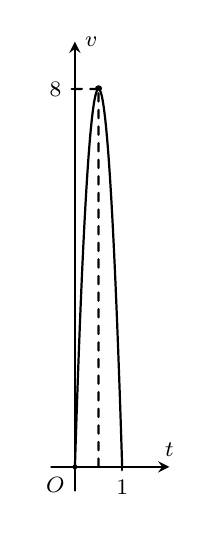
\begin{tikzpicture}[>=stealth, font=\footnotesize, line join=round, line cap=round, thick, smooth, samples=250, scale=0.6]
% Vẽ 2 trục, điền các số lên trục
 \draw[->] (-0.5,0)--(0,0) node[below left]{$O$}--(2,0) node[above]{$t$}; %định dạng trục Ox
\foreach \x in {1}
\draw[shift={(\x,0)},color=black] (0pt,2pt)--(0pt,-2pt) 
node[below] { $\x$};
\draw[->,color=black] (0,-0.5)--(0,9) node[right]{$v$};  %định dạng trục Oy
\foreach \y in {8}
\draw[shift={(0,\y)},color=black] (2pt,0pt) -- (-2pt,0pt) 
node[left] {$\y$};
\clip(-1,-1) rectangle (2,9); %vùng đồ thị
%\draw[gray!50,thin,opacity=.5] (-1,-1) grid (4,10); %ô vuông
%Vẽ đồ thị
\draw[smooth,samples=50,domain=0:1] 
plot(\x,{-32*(\x)^2+32*(\x)});
% Vẽ thêm mấy cái râu ria
\draw[dashed] (1/2,0)--(1/2,8) circle(1.5pt)--(0,8);
%Vẽ dấu chấm tròn 
\fill (0cm,0cm) circle (1.5pt); 
\end{tikzpicture} 
}
\shortans{$4,5$}
	\loigiai{
\immini{
	Gọi parabol là $\left(P\right) \colon y = ax^2 + bx + c$. Từ hình vẽ ta có $\left(P\right)$ đi qua $O\left(0;0\right)$, $A \left(1;0\right)$ và điểm $I\left(\dfrac{1}{2};8\right)$.\\
	Ta có hệ: $\heva{&c=0\\&a+b+c=0\\&\dfrac{a}{4}+\dfrac{b}{2}+c = 8} \Leftrightarrow \heva{&a=-32\\&b=32\\&c=0.}$\\
	Suy ra $\left(P\right) \colon y = -32x^2 + 32x$.\\
	Vậy quãng đường người đó đi được là $s = \displaystyle\int\limits_0^{\tfrac{3}{4}} \left(-32x^2 + 32x \right) \mathrm{\,d}x = 4{,}5$ (km).
}
{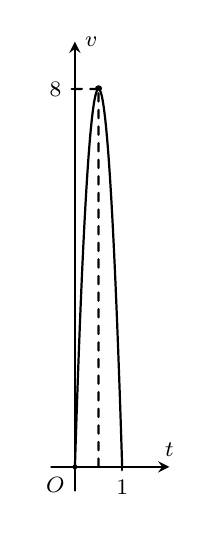
\begin{tikzpicture}[>=stealth, font=\footnotesize, line join=round, line cap=round, thick, smooth, samples=250, scale=0.6]
		% Vẽ 2 trục, điền các số lên trục
		\draw[->] (-0.5,0)--(0,0) node[below left]{$O$}--(2,0) node[above]{$t$}; %định dạng trục Ox
		\foreach \x in {1}
		\draw[shift={(\x,0)},color=black] (0pt,2pt)--(0pt,-2pt) 
		node[below] { $\x$};
		\draw[->,color=black] (0,-0.5)--(0,9) node[right]{$v$};  %định dạng trục Oy
		\foreach \y in {8}
		\draw[shift={(0,\y)},color=black] (2pt,0pt) -- (-2pt,0pt) 
		node[left] {$\y$};
		\clip(-1,-1) rectangle (2,9); %vùng đồ thị
		%\draw[gray!50,thin,opacity=.5] (-1,-1) grid (4,10); %ô vuông
		%Vẽ đồ thị
		\draw[smooth,samples=50,domain=0:1] 
		plot(\x,{-32*(\x)^2+32*(\x)});
		% Vẽ thêm mấy cái râu ria
		\draw[dashed] (1/2,0)--(1/2,8) circle(1.5pt)--(0,8);
		%Vẽ dấu chấm tròn 
		\fill (0cm,0cm) circle (1.5pt); 
\end{tikzpicture} }
	}
\end{ex}

\begin{ex}%Cau22D%[2D4V2-6]
Một vật chuyển động trong $4$ giờ với vận tốc $v$ (km/h) phụ thuộc thời gian $t$ (h) có đồ thị của vận tốc như hình bên. Trong khoảng thời gian $3$ giờ kể từ khi bắt đầu chuyển động, đồ thị đó là một phần của đường parabol có đỉnh $I \left(2;9\right)$ với trục đối xứng song song với trục tung, khoảng thời gian còn lại đồ thị là một đoạn thẳng song song với trục hoành. Tính quãng đường $s$ mà vật di chuyển được trong $4$ giờ đó (đơn vị tính bằng km).
\begin{center}
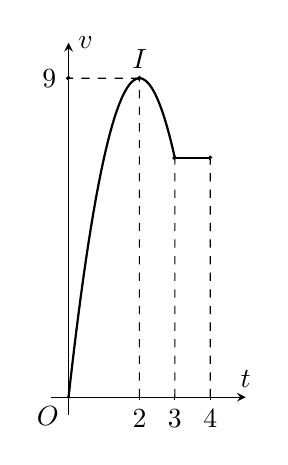
\begin{tikzpicture}[>=stealth,scale=0.45]
% Vẽ 2 trục, điền các số lên trục
 \draw[->] (-0.5,0)--(0,0) node[below left]{$O$}--(5,0) node[above]{$t$};
\foreach \x in {2,3,4}
\draw[shift={(\x,0)},color=black] (0pt,2pt)--(0pt,-2pt) 
node[below] { $\x$};
\draw[->,color=black] (0,-0.5)--(0,10) node[right]{$v$};
\foreach \y in {9}
\draw[shift={(0,\y)},color=black] (2pt,0pt) -- (-2pt,0pt) 
node[left] {$\y$};
\clip(-1,-1) rectangle (5,10); %vùng đồ thị
%\draw[gray!50,thin,opacity=.5] (-1,-1) grid (4,10); %ô vuông
%Vẽ đồ thị
\draw[smooth,samples=100,domain=0:3, font=\footnotesize, line join=round, line cap=round, thick, smooth] 
plot(\x,{(-9/4)*(\x)^2+9*(\x)});
\draw[smooth,samples=100, font=\footnotesize, line join=round, line cap=round, thick, smooth,domain=3:4] 
plot(\x,{27/4});
% Vẽ thêm mấy cái râu ria
\draw[dashed] (3,0)--(3,27/4) circle(1.5pt);  \draw[dashed] (2,0)--(2,9) circle(1.5pt) node[above]{$I$}--(0,9) circle(1.5pt); \draw[dashed] (4,0)--(4,27/4) circle(1.5pt);
%Vẽ dấu chấm tròn 
\fill (0cm,0cm) circle (1.5pt); 
\end{tikzpicture} 
\end{center}
\shortans{$27$}
	\loigiai{
	Gọi $\left(P\right) \colon y = ax^2+bx+c$.\\
	Vì $\left(P\right)$ qua $O\left(0;0\right)$ và có đỉnh $I\left(2;9\right)$ nên dễ tìm được phương trình là $y = \dfrac{-9}{4}x^2 + 9x$.\\
	Ngoài ra tại $x=3$ ta có $y = \dfrac{27}{4}$.\\
	Vậy quãng đường cần tìm là: $S = \displaystyle\int\limits_0^3 \left(\dfrac{-9}{4}x^2 +9x \right) \mathrm{\,d}x + \displaystyle\int\limits_3^4 \dfrac{27}{4} \mathrm{\,d}x = 27$ (km).
	}
\end{ex}

\begin{ex}%Cau23D%[2D4V2-6]
Một vật chuyển động trong $6$ giờ với vận tốc $v$ (km/h) phụ thuộc vào thời gian $t$ (h) có đồ thị như hình bên dưới. Trong khoảng thời gian $2$ giờ từ khi bắt đầu chuyển động, đồ thị là một phần đường Parabol có đỉnh $I\left(3;9\right)$ và có trục đối xứng song song với trục tung. Khoảng thời gian còn lại, đồ thị vận tốc là một đường thẳng có hệ số góc bằng $\dfrac{1}{4}$. Tính quảng đường $s$ mà vật di chuyển được trong $6$ giờ? (đơn vị tính bằng km, làm tròn đến chữ số thập phân thứ nhất).
\begin{center}
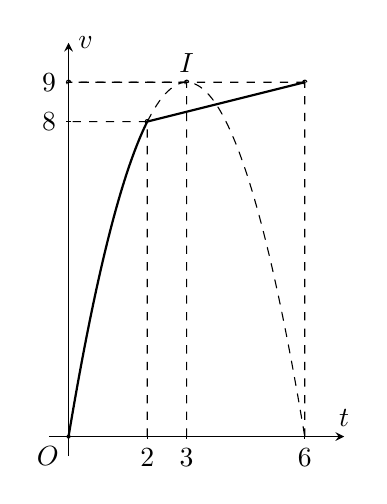
\begin{tikzpicture}[>=stealth,scale=0.5]
% Vẽ 2 trục, điền các số lên trục
 \draw[->] (-0.5,0)--(0,0) node[below left]{$O$}--(7,0) node[above]{$t$}; %định dạng trục Ox
\foreach \x in {2,3,6}
\draw[shift={(\x,0)},color=black] (0pt,2pt)--(0pt,-2pt) 
node[below] { $\x$};
\draw[->,color=black] (0,-0.5)--(0,10) node[right]{$v$};  %định dạng trục Oy
\foreach \y in {8,9}
\draw[shift={(0,\y)},color=black] (2pt,0pt) -- (-2pt,0pt) 
node[left] {$\y$};
\clip(-1,-1) rectangle (7,10); %vùng đồ thị
%\draw[gray!50,thin,opacity=.5] (-1,-1) grid (4,10); %ô vuông
%Vẽ đồ thị
\draw[smooth,samples=100,domain=0:2,font=\footnotesize, line join=round, line cap=round, thick] 
plot(\x,{(-1)*(\x)^2+6*(\x)});
\draw[smooth,domain=2:6, line join=round, line cap=round,dashed] 
plot(\x,{(-1)*(\x)^2+6*(\x)});
\draw[smooth,samples=100,domain=2:6,font=\footnotesize, line join=round, line cap=round, thick] 
plot(\x,{(1/4)*(\x)+15/2});
% Vẽ thêm mấy cái râu ria
\draw[dashed] (3,0)--(3,9) circle(1.5pt) node[above]{$I$}--(0,9) circle(1.5pt); 
\draw[dashed] (2,0)--(2,8) circle(1.5pt) --(0,8);
\draw[dashed] (6,0)--(6,9) circle(1.5pt) --(0,9);
%Vẽ dấu chấm tròn 
\fill (0cm,0cm) circle (1.5pt); 
\end{tikzpicture}
\end{center}
\shortans{$43{,}3$}
	\loigiai{
	Vì Parabol đi qua $O\left(0;0\right)$ và có tọa độ đỉnh $I\left(3;9\right)$ nên thiết lập được phương trình Parabol là $\left(P\right) \colon y = v\left(t\right) = -t^2+6t$; $\forall t \in \left[0;2\right]$.\\
	Sau $2$ giờ đầu thì hàm vận tốc có dạng là hàm bậc nhất $y = \dfrac{1}{4}t + m$, dựa trên đồ thị ta thấy đi qua điểm có tọa độ $\left(6;9\right)$ nên thế vào hàm số và tìm được $m = \dfrac{15}{2}$.\\
Nên hàm vận tốc từ giờ thứ $2$ đến giờ thứ $6$ là: $y = \dfrac{1}{4}t + \dfrac{15}{2},\forall t \in \left[2;6\right]$.\\
	Quảng đường vật đi được bằng tổng đoạn đường $2$ giờ đầu và đoạn đường $4$ giờ sau.
	$$S = S_1 +S_2 = \displaystyle\int\limits_0^2 \left(-t^2+6t\right) \mathrm{\,d}t + \displaystyle\int\limits_2^6 \left(\dfrac{1}{4}t+\dfrac{15}{2} \right) \mathrm{\,d}t = \dfrac{130}{3} \approx 43{,}3 \left(\text{km}\right).$$
	}
\end{ex}

\begin{ex}%Cau24D%[2D4H2-6]
\immini{Một người chạy trong thời gian $1$ giờ, với vận tốc $v$ (km/h) phụ thuộc vào thời gian $t$ (h) có đồ thị là một phần của parabol có đỉnh $I \left(\dfrac{1}{2};8\right)$ và trục đối xứng song song với trục tung như hình vẽ. Tính quãng đường $S$ người đó chạy được trong thời gian $45$ phút, kể từ khi bắt đầu chạy (đơn vị tính bằng km).
}{
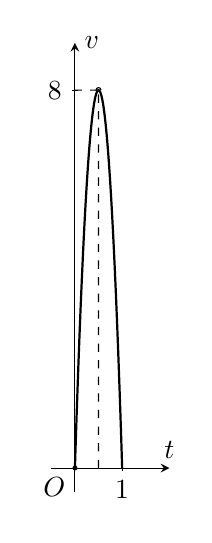
\begin{tikzpicture}[>=stealth, scale=0.6]
% Vẽ 2 trục, điền các số lên trục
 \draw[->] (-0.5,0)--(0,0) node[below left]{$O$}--(2,0) node[above]{$t$}; %định dạng trục Ox
\foreach \x in {1}
\draw[shift={(\x,0)},color=black] (0pt,2pt)--(0pt,-2pt) 
node[below] { $\x$};
\draw[->,color=black] (0,-0.5)--(0,9) node[right]{$v$};  %định dạng trục Oy
\foreach \y in {8}
\draw[shift={(0,\y)},color=black] (2pt,0pt) -- (-2pt,0pt) 
node[left] {$\y$};
\clip(-1,-1) rectangle (2,9); %vùng đồ thị
\draw[smooth,samples=50,domain=0:1, font=\footnotesize, line join=round, line cap=round, thick] 
plot(\x,{-32*(\x)^2+32*(\x)});
\draw[dashed] (1/2,0)--(1/2,8) circle(1.5pt)--(0,8);
\fill (0cm,0cm) circle (1.5pt); 
\end{tikzpicture}
}
\shortans{$4{,}5$}
	\loigiai{
		Trước hết ta tìm công thức biểu thị vận tốc theo thời gian, giả sử $v\left(t\right) = at^2+bt+c$.\\  .
Khi đó dựa vào hình vẽ ta có hệ phương trình\\
$$\heva{&c=0\\&a\left(\dfrac{1}{2}\right)^2+b\left(\dfrac{1}{2}\right)+c =8\\&a+b+c=0} \Leftrightarrow \heva{&a=-32\\&b=32\\&c=0.}$$
Do đó quãng đường người đó đi được sau $45$ phút là $S = \displaystyle\int\limits_0^{\tfrac{45}{60}} \left(32t-32t^2\right) \mathrm{\,d}t = 4{,}5$ (km).
	}
\end{ex}

\begin{ex}%Cau25D%[2D4H2-6]
Một vật chuyển động trong $4$ giờ với vận tốc $v$ (km/h) phụ thuộc thời gian $t$ (h) có đồ thị là một phần của đường parabol có đỉnh $I\left(1;1\right)$ và trục đối xứng song song với trục tung như hình bên. Tính quãng đường $s$ mà vật di chuyển được trong $4$ giờ kể từ lúc xuất phát (làm tròn đến chữ số thập phân thứ nhất).
\begin{center}
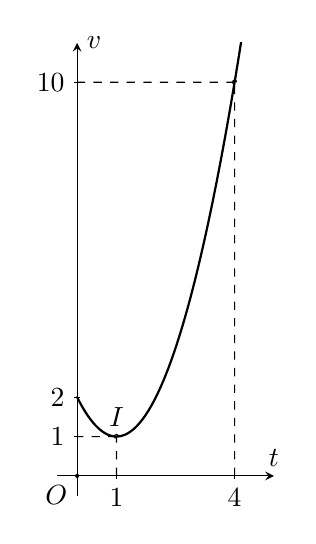
\begin{tikzpicture}[>=stealth,scale=0.5]
% Vẽ 2 trục, điền các số lên trục
 \draw[->] (-0.5,0)--(0,0) node[below left]{$O$}--(5,0) node[above]{$t$};
\foreach \x in {1,4}
\draw[shift={(\x,0)},color=black] (0pt,2pt)--(0pt,-2pt) 
node[below] { $\x$};
\draw[->,color=black] (0,-0.5)--(0,11) node[right]{$v$};
\foreach \y in {1,2,10}
\draw[shift={(0,\y)},color=black] (2pt,0pt) -- (-2pt,0pt) 
node[left] {$\y$};
\clip(-1,-1) rectangle (5,11); %vùng đồ thị
\draw[smooth,samples=100,domain=0:10, font=\footnotesize, line join=round, line cap=round, thick] 
plot(\x,{(\x)^2-2*(\x)+2});
% Vẽ thêm mấy cái râu ria
\draw[dashed] (4,0)--(4,10) circle(1.5pt)--(0,10);  \draw[dashed] (1,0)--(1,1) circle(1.5pt) node[above]{$I$}--(0,1);
%Vẽ dấu chấm tròn 
\fill (0cm,0cm) circle (1.5pt); 
\end{tikzpicture} 
\end{center}
\shortans{$13{,}3$}
	\loigiai{Hàm biểu diễn vận tốc có dạng $v\left(t\right) = at^2+bt+c$. Dựa vào đồ thị ta có
	$$\heva{&c=2\\&-\dfrac{b}{2a}=1\\&a+b+c=1} \Leftrightarrow \heva{&a=1\\&b=-2\\&c=2} \Leftrightarrow v\left(t\right) = t^2 -2t+2.$$
	Với $t=4 \Rightarrow v\left(4\right) = 10$ (thõa mãn).\\
	Từ đó $s = \displaystyle\int\limits_0^4 \left(t^2-2t+2\right) \mathrm{\,d}t = \dfrac{40}{3} \approx 13{,}3$ (km).
	}
\end{ex}

\begin{ex}%Cau26D%[2D4V2-6]
Chất điểm chuyển động theo quy luật vận tốc $v\left(t\right)$ (m/s) có dạng đường Parapol khi $0 \leq t\leq 5$ (s) và $v\left(t\right)$ có dạng đường thẳng khi $5 \leq t \leq 10$ (s). Cho đỉnh Parapol là $I\left(2;3\right)$. Hỏi quãng đường đi được chất điểm trong thời gian $0 \leq t \leq 10$ (s) là bao nhiêu mét? (làm tròn đến hàng đơn vị)
\begin{center}
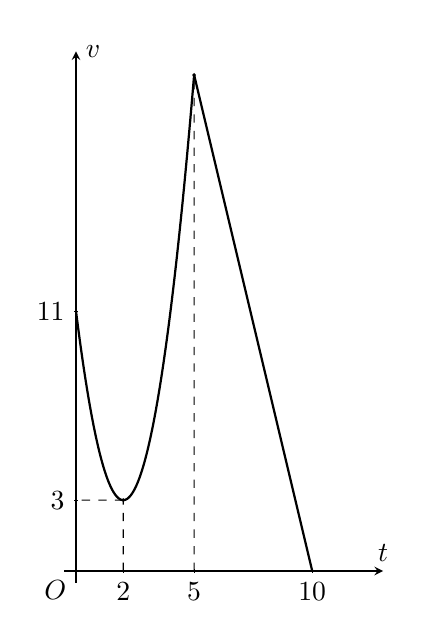
\begin{tikzpicture}[>=stealth,scale=0.3]
% Vẽ 2 trục, điền các số lên trục
 \draw[->] (-0.5,0)--(0,0) node[below left]{$O$}--(13,0) node[above]{$t$};
\foreach \x in {2,5,10}
\draw[shift={(\x,0)},color=black] (0pt,2pt)--(0pt,-2pt) 
node[below] { $\x$};
\draw[->,color=black] (0,-0.5)--(0,22) node[right]{$v$};
\foreach \y in {3,11}
\draw[shift={(0,\y)},color=black] (2pt,0pt) -- (-2pt,0pt) 
node[left] {$\y$};
\clip(-1,-1) rectangle (11,23); %vùng đồ thị
\draw[smooth,samples=100,domain=0:5, font=\footnotesize, line join=round, line cap=round, thick] 
plot(\x,{2*(\x)^2-8*(\x)+11});
\draw[smooth,samples=100,domain=5:10, font=\footnotesize, line join=round, line cap=round, thick] 
plot(\x,{(-21/5)*(\x)+42});
% Vẽ thêm mấy cái râu ria
\draw[dashed] (5,0)--(5,21) circle(1.5pt);  \draw[dashed] (2,0)--(2,3) circle(1.5pt)--(0,3);
%Vẽ dấu chấm tròn 
\fill (0cm,0cm) circle (1.5pt); 
\end{tikzpicture}
\end{center}
\shortans{$91$}
	\loigiai{
	Gọi Parapol $\left(P\right) \colon y = ax^2+bx+c$ khi $0 \leq t \leq 5 \left(s\right)$.\\  
Do $\left(P\right) \colon y = ax^2+bx+c$ đi qua $I\left(3;2\right)$; $A \left(0;11\right)$ nên
$$\heva{&4a+2b+c=3\\&c=11\\&4a+b=0} \Rightarrow \heva{&a=2\\&b=-8\\&c=11.}$$
Khi đó quãng đường vật di chuyển trong khoảng thời gian từ $0 \leq t \leq 5$ (s) là
$$S_1 = \displaystyle\int\limits_0^5 \left(2x^2 - 8x +11\right) \mathrm{\,d}x = \dfrac{115}{3} \left(\text{m}\right).$$
	Ta có $f\left(5\right) = 21$.\\
	Gọi $d \colon y = ax+b$ khi $5 \leq t \leq 10$ (s), do $d$ đi qua điểm $B\left(5;21\right)$ và $C\left(10;0\right)$ nên
	$$\heva{&5a+b=11\\&10a+b=0} \Rightarrow \heva{&a=-\dfrac{21}{5}\\&b=42.}$$
Khi đó quãng đường vật di chuyển trong khoảng thời gian từ $5 \leq t \leq 10$ (s) là:
$$S_2 = \displaystyle\int\limits_5^{10} \left(-\dfrac{21}{5}x+42\right) \mathrm{\,d}x = \dfrac{105}{2} \left(\text{m}\right).$$
Quãng đường đi được chất điểm trong thời gian  $0 \leq t \leq 10$ (s) là:
$$S = \dfrac{115}{3}+\dfrac{105}{2}= \dfrac{545}{6} \approx 91 \left(\text{m}\right).$$
	}
\end{ex}
\Closesolutionfile{ans}
% \indapan{6}{ans/ans-2C4B2CD3-KQ}